\documentclass[12pt,addpoints]{uofmexamNoHeader}

\usepackage{enumitem}

%\makeatletter
%%%%%%%%%%%%%%%%%
\PassOptionsToPackage{force}{filehook}
\usepackage{tikz}
%\usetikzlibrary{shapes}
\usetikzlibrary{plotmarks}
\usetikzlibrary{positioning}% To get more advances positioning options
\usetikzlibrary{arrows}
\usetikzlibrary{patterns}

\usetikzlibrary{calc}
\usepackage{dsfont}
\usetikzlibrary{calc}
\tikzset{smalldot/.style={circle,draw=black,fill=black,inner sep = 1pt}}

\usetikzlibrary{calc}
\tikzset{smalldot/.style={circle,draw=black,fill=black,inner sep = 1.5pt}}
\tikzset{opendot/.style={circle,draw=black,fill=white,inner sep = 1.5pt}}

\usetikzlibrary{shapes,arrows}
\usetikzlibrary{positioning}
\tikzstyle{cloud} = [draw, ellipse,fill=red!20, node distance=0.87cm,
minimum height=2em]
\tikzstyle{line} = [draw, -latex']
\usetikzlibrary{shapes.symbols,shapes.callouts,patterns}
\usetikzlibrary{calc,fit}
\usetikzlibrary{backgrounds}

\def\IC{\mathbb{C}}
\def\IF{\mathbb{F}}
\def\II{\mathbb{I}}
\def\IN{\mathbb{N}}
\def\IR{\mathbb{R}}
\def\IZ{\mathbb{Z}}

\def\b0{\mathbf{0}}
\def\bb{\mathbf{b}}
\def\be{\mathbf{e}}
\def\bi{\mathbf{i}}
\def\bj{\mathbf{j}}
\def\bk{\mathbf{k}}
\def\bu{\mathbf{u}}
\def\bv{\mathbf{v}}
\def\bw{\mathbf{w}}
\def\bx{\mathbf{x}}
\def\by{\mathbf{y}}
\def\bz{\mathbf{z}}

\def\B{\mathcal{B}}
\def\C{\mathcal{C}}
\def\E{\mathcal{E}}
\def\L{\mathcal{L}}
\def\M{\mathcal{M}}
\def\N{\mathcal{N}}

\def\ker{\ensuremath{\text{ker}}}


\newtheorem{theorem}{Theorem}
\newtheorem{definition}[theorem]{Definition}

\newcommand{\dist}[1]{\mathsf{dist}[#1]}
\newcommand{\prev}[1]{\mathsf{prev}[#1]}
\def\alt{\text{\tt alt}\ }
\def\length{\text{\tt length}}


\examinfo{%
	type={ASSIGNMENT 8},	% Optional; leave blank or do not specify to omit.
	coursenumber={MATH 2740},	% include section, unless this is a multisection exam.
	%crn={CRN},	% Optional; leave blank or do not specify to omit.
	%examiner={Examiner},	% Optional; leave blank or do not specify to omit
	duration={1 week},
	date={Due 11 October},
	time={12:00},
	crowdmark=duplex,	% single sided is the default (no =duplex); use crowdmark=duplex for two-sided.
	}

% uncomment \printanswers for a solution key
%\printanswers

\pointsinmargin
\bracketedpoints

\geometry{letterpaper,bottom=0.5in}	% legalpaper is the default.

%%%%%%%%%%%%%%%%%%%%%%%%%%%%%%%%%%%%%%%%%%%%%
\begin{document}

\begin{center}
	\large
	\textbf{AARMS 2023 Summer School\\20--30 August 2023\\Metapopulations \& introductions models problem set}\\[0.5cm]
\end{center}

\begin{questions}

%%%%%%%%%%%%%%%%%%%%%%%%%%%%%%%%%%%%%%%%%%%%%
\question[10]
Consider the Kermack-McKendrick SIR \emph{epidemic} model
\begin{center}
    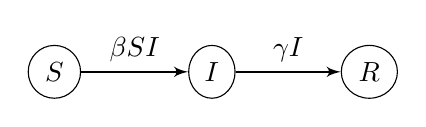
\begin{tikzpicture}[auto,
        cloud/.style={minimum width={width("-12")+2pt},
            draw, ellipse},
        connected/.style={dotted,-}]
        %% Vertices
        \node [cloud] at (0,0) (S) {$S$};
        \node [cloud] at (2,0) (I){$I$};
        \node [cloud] at (4,0) (R){$R$};
        %% Arcs
        \path [line, thick] (S) to node [midway, above] (TextNode) {$\beta SI$} (I);
        \path [line, thick] (I) to node [midway, above] (TextNode) {$\gamma I$} (R);
    \end{tikzpicture}
\end{center}
and the \emph{endemic} SIR model with demography
\begin{center}
    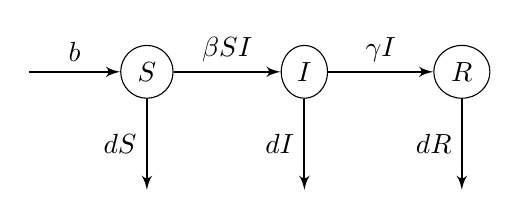
\begin{tikzpicture}[auto,
        cloud/.style={minimum width={width("-12")+2pt},
            draw, ellipse},
        connected/.style={dotted,-}]
        %% Vertices
        \node [cloud] at (0,0) (S) {$S$};
        \node [cloud] at (2,0) (I){$I$};
        \node [cloud] at (4,0) (R){$R$};
        %% Arcs
        \path [line, thick] (-1.5,0) to node [midway, above] (TextNode) {$b$} (S);
        \path [line, thick] (S) to node [midway, above] (TextNode) {$\beta SI$} (I);
        \path [line, thick] (S) to node [midway, left] (TextNode) {$dS$} (0,-1.5);
        \path [line, thick] (I) to node [midway, above] (TextNode) {$\gamma I$} (R);
        \path [line, thick] (I) to node [midway, left] (TextNode) {$dI$} (2,-1.5);
        \path [line, thick] (R) to node [midway, left] (TextNode) {$dR$} (4,-1.5);
    \end{tikzpicture}
\end{center}

\begin{parts}
    \part Write simple, $|\mathcal{P}|$-metapopulation models based on each model, using explicit movement as well as implicit coupling. The latter means that coupling is \emph{not} through the movement of individuals between locations, but through the incidence function, i.e., mass action incidence in patch $p$ takes the form
    \[
        S_p\left(\sum_{q\in\mathcal{P}}\beta_{qp}I_q\right),
    \]
    with $\beta_{qp}$ the contact parameter (``influence'') of infectious individuals in patch $q$ on susceptible individuals in patch $p$.
    \part From now on, consider only the two models with explicit movement. Compute the DFE (beware in the case of the epidemic model) and $\mathcal{R}_0$.
    \part In the endemic case, it is easy to compute the endemic equilibrium in the single population case, by writing the equation for the dynamics of $I(t)$ as
    \[
        I' = \left(\beta S-(\gamma+d)\right)I.
    \]
    Does this work in the metapopulation case? Why/why not?
    \part Modifying the code I gave in the CODE directory, write code to simulate both systems.
    \part Write code to simulate both systems as continuous-time Markov chains in a two-patch situation.
    \part (Bonus) Write code to simulate the models as CTMC in the case of an arbitrary number of patches.
    \part Investigate introductions in the two-patch context, by using the capacity of {\tt ssa} in {\tt GillespieSSA2} to return events.
\end{parts}


\begin{solution}
\end{solution}




\end{questions}
\end{document}